\documentclass[preprint,11pt,authoryear]{elsarticle}
\pdfoutput=1
\pdfminorversion=4 %had problems submitting a v1.5 pdf file with J Neurosci Methods
\usepackage{graphicx}
\usepackage{amsmath}
\usepackage{esint}
\usepackage{amssymb}
\usepackage{lineno}
\usepackage[T1]{fontenc}
\usepackage[utf8]{inputenc}
\usepackage[english]{babel}
\usepackage[]{algorithm}
\usepackage[noend]{algpseudocode}
%% natbib.sty is loaded by default. However, natbib options can be
%% provided with \biboptions{...} command. Following options are
%% valid:

%%   round  -  round parentheses are used (default)
%%   square -  square brackets are used   [option]
%%   curly  -  curly braces are used      {option}
%%   angle  -  angle brackets are used    <option>
%%   semicolon  -  multiple citations separated by semi-colon
%%   colon  - same as semicolon, an earlier confusion
%%   comma  -  separated by comma
%%   numbers-  selects numerical citations
%%   super  -  numerical citations as superscripts
%%   sort   -  sorts multiple citations according to order in ref. list
%%   sort&compress   -  like sort, but also compresses numerical citations
%%   compress - compresses without sorting
%%
%% \biboptions{comma,round}

% \biboptions{}

\bibliographystyle{elsarticle-harv}
\biboptions{square}

\renewcommand\familydefault{\sfdefault}
\usepackage[scaled]{helvet}

\usepackage{units}
\usepackage[usenames, dvipsnames]{xcolor}

\usepackage{soul}
\usepackage{placeins}

\usepackage{nameref}
\usepackage[pdftex,breaklinks=true,colorlinks=true,linkcolor=blue,citecolor=blue,urlcolor=blue,filecolor=blue,pdffitwindow,backref=true,pagebackref=false,bookmarks=true,bookmarksopen=true,bookmarksnumbered=true]{hyperref}
\usepackage[plain]{fancyref}
\usepackage{array}
\usepackage{multirow}

% Text layout
%\hoffset 2 cm
\topmargin 0.0cm
\oddsidemargin 0.5cm
\evensidemargin 0.5cm
\textwidth 16cm 
\textheight 21cm

%custom color for \hlc
\newcommand{\hlc}[2][yellow]{ {\sethlcolor{#1} \hl{#2}} }
\newcommand{\hlb}[2][blue]{ {\sethlcolor{#1} \hl{#2}} }
\newcommand{\hlr}[2][Maroon]{ {\sethlcolor{#1} \hl{#2}} }
\newcommand{\hlj}[2][OliveGreen]{ {\sethlcolor{#1} \hl{#2}} }
\newcommand{\hlR}[2][red]{ {\sethlcolor{#1} \hl{#2}} }

%boxes and highlight color for text updates, personified!
\newcommand{\ghnote}[1]{\color{white}{\hlb{GH: #1 }}\color{black}}
\newcommand{\ghtxt}[1]{{\color{blue}#1}}
\newcommand{\gtenote}[1]{\color{white}{\hlR{GTE: #1 }}\color{black}}
\newcommand{\gen}[1]{\color{white}{\hlR{GTE: #1 }}\color{black}}
\newcommand{\gtetxt}[1]{{\color{red}#1}}
\newcommand{\gex}[1]{{\color{red}#1}}
\newcommand{\genn}[1]{{\color{orange}#1}}

\newcommand{\tvnnote}[1]{\color{white}{\hlj{TVN: #1 }}\color{black}}
\newcommand{\tvntxt}[1]{{\color{OliveGreen}#1}}

%fancy ref formatting
\Frefformat{plain}{\fancyreffiglabelprefix}{Fig~#1}
\newcommand*{\Frefsecshortname}{Section}%
\Frefformat{plain}{\fancyrefseclabelprefix}{\Frefsecshortname~#1}
\Frefformat{plain}{\fancyrefeqlabelprefix}{Eq~(#1)}

%tables as in Nordlie et al. (2009)
\usepackage{tabularx}
\usepackage{colortbl}
\usepackage{morefloats}

%table formatting
\newcommand{\modelhdr}[3]{%
   \multicolumn{#1}{|l|}{%
     \color{white}\cellcolor[gray]{0.0}%
     \textbf{\makebox[0pt]{#2}\hspace{0.5\linewidth}\makebox[0pt][c]{#3}}%
   }%
}
\newcommand{\parameterhdr}[3]{%
   \multicolumn{#1}{|l|}{%
     \color{black}\cellcolor[gray]{0.8}%
     \textbf{\makebox[0pt]{#2}\hspace{0.5\linewidth}\makebox[0pt][c]{#3}}%
   }%
}
\def\tabspace{0.5ex}

\usepackage{float}
\floatstyle{plaintop}
\restylefloat{table}

\journal{nobody}


% redefinition of \author{•} because of bug (reset of \@corref missing), taken from:
% http://tex.stackexchange.com/questions/116515/elsarticle-frontmatter-corresponding-author
\makeatletter
\def\@author#1{\g@addto@macro\elsauthors{\normalsize%
    \def\baselinestretch{1}%
    \upshape\authorsep#1\unskip\textsuperscript{%
      \ifx\@fnmark\@empty\else\unskip\sep\@fnmark\let\sep=,\fi
      \ifx\@corref\@empty\else\unskip\sep\@corref\let\sep=,\fi
      }%
    \def\authorsep{\unskip,\space}%
    \global\let\@fnmark\@empty
    \global\let\@corref\@empty  %% Added
    \global\let\sep\@empty}%
    \@eadauthor={#1}
}
\makeatother

% - mine pakker -
\usepackage[exponent-product = \cdot]{siunitx}
\usepackage[colorinlistoftodos]{todonotes}
\usepackage[normalem]{ulem} % strikethroughs \sout{Hello World}
\usepackage{caption}
\usepackage{booktabs} % to make nice tables
\graphicspath{{Figures/}} %Setting the graphicspath
\usepackage{caption}
\usepackage{subcaption}

% - mine kommandoer - 


\begin{document}

\begin{frontmatter}

%% Title, authors and addresses

\title{Computing extracellular electrical potentials from in silico neuronal simulations\tvnnote{How about the more general ``Computing brain signals from neural simulations''}} 

%% use the tnoteref command within \title for footnotes;
%% use the tnotetext command for the associated footnote;
%% use the fnref command within \author or \address for footnotes;
%% use the fntext command for the associated footnote;
%% use the corref command within \author for corresponding author footnotes;
%% use the cortext command for the associated footnote;
%% use the ead command for the email address,
%% and the form \ead[url] for the home page:
%%
%% \title{Title\tnoteref{label1}}
%% \tnotetext[label1]{}
%% \author{Name\corref{cor1}\fnref{label2}}
%% \ead{email address}
%% \ead[url]{home page}
%% \fntext[label2]{}
%% \cortext[cor1]{}
%% \address{Address\fnref{label3}}
%% \fntext[label3]{}

%% use optional labels to link authors explicitly to addresses:
%% \author[label1,label2]{<author name>}
%% \address[label1]{<address>}
%% \address[label2]{<address>}

\author{Geir Halnes\fnref{label1,label2}}
\author{Torbj\o{}rn V. Ness \fnref{label1,label2}}
\author{Solveig N\ae{}ss\fnref{label2}}
\author{Klas Pettersen \fnref{label3}}
\author{Gaute T. Einevoll\corref{cor1}\fnref{label1,label2,label4}}

\address[label1]{Faculty of Science and Technology, Norwegian University of Life Sciences, {{\AA}}s, Norway}
\address[label2]{Center for Integrative Neuroplasticity, University of Oslo, Oslo, Norway}
\address[label3]{Norwegian Artificial Intelligence Research Consortium, Oslo, Norway}
\address[label4]{Department of Physics, University of Oslo, Oslo, Norway}

\cortext[cor1]{correspondence: \href{geir.halnes@nmbu.no}{gaute.einevoll@nmbu.no}}

%%%%%%%%%%%%%%%%%%%%%%%%%%%%%%%%%%%%%%%%%%%%%%%%%%
%%%%%%%%%%%%%%%%%%%%%%%%%%%%%%%%%%%%%%%%%%%%%%%%%%


\begin{abstract}
%% Text of abstract
\ghnote{Vet ikke hva forfatterordningen skal vaere, men vi faar se det an etter hvert, og bestemme utifra hvem som har jobbet mest med manus. For oeyeblikket leder jeg, men jeg tror jeg satser paa at kanskje Torbjoern fosser forbi etter hvert.}
\tvnnote{Just to be sure: If we make figures for this chapter, we have the right to re-use those wherever we like?}
\tvnnote{Giugliano: max 15-20 pages, by February 2020 }
\end{abstract}

\begin{keyword}
extracellular potentials \sep LFP \sep EEG \sep ECoG \sep electrodiffusion
%% keywords here, in the form: keyword \sep keyword

%% MSC codes here, in the form: \MSC code \sep code
%% or \MSC[2008] code \sep code (2000 is the default)
\end{keyword}

\end{frontmatter}

\tableofcontents

%%%%%%%%%%%%%%%%%%%%%%%%%%%%%%%%%%%%%%%%%%%%%%%%%%
%%%%%%%%%%%%%%%%%%%%%%%%%%%%%%%%%%%%%%%%%%%%%%%%%%
%% Start line numbering here if you want
\linenumbers

\section{Introduction}
\label{sec:introduction}

\ghnote{First something about why we are interested in electrical fields and some historical perspectives. Perhaps Gaute should write this.}

\ghnote{End intro with bridge to theory-section. Probably we should add some older references to VC-theory?}

Very important to model what you measure, and measure what you model \citep{Einevoll2019, Maki-marttunen2019}

Electrical currents in the brain are mediated by the movement of ions, and it is these currents that a recording electrode pick up.  A net electrical current through the extracellular space of the brain could in principle include several components, such as (1) a drift component (ions move due to migration in electrical fields, (2) a diffusion component (ions move due to diffusion), (3) an advective component (ions move because the extracellular fluid is flowing and dragging them along), and (4) a displacement component (ions pile up locally and give rise to a temporal change in the charge density). Since the extracellular bulk fluid has very fast relaxation times and is very close to electroneutral, the latter two current components (3-4) are extremely small and can be neglected \citep{Grodzinsky2011, Gratiy2017}. The diffusive component (3) is acknowledged to play an important role for voltage dynamics on a tiny spatial scale, such as in synaptic clefts or in the close vicinity of neuronal membrane, where ion concentrations can change dramatically within very short time \citep{Savtchenko2017, Pods2017}. At the level of tissue however, it is commonly believed that the diffusive current is much smaller than the migratory current\tvnnote{migratory current is a new term to me. use 'drift' as under (1)? Wikipedia: ``Electromigration is the transport of material caused by the gradual movement of the ions in a conductor due to the momentum transfer between conducting electrons and diffusing metal atoms''. Are we sure about this term?}, and diffusion is therefore \tvntxt{typically} neglected %when volume conductor (VC) theory is used to compute extracellular potentials 
\citep{Holt1999, Pettersen2008a}. 
This is often a useful approximation, since modeling of electrodiffusive processes is computationally expensive and may not be feasible for large and complex systems. However, \tvntxt{if} %when
concentration gradients are present, diffusive currents \tvntxt{can be expected to} %will 
induce shifts in the \tvntxt{measurable} extracellular potential %also on the tissue level 
\citep{Halnes2016, Halnes2017, Solbra2018}, and in scenarios involving dramatic shifts in extracellular concentrations, such as spreading depression and related pathologies, diffusive effects are likely to be \tvntxt{of key importantance for shaping} the extracellular potential \citep{Almeida2004, OConnell2016}.

We start this book chapter by giving an overview of the theory used for forward modellng of extracellular potentials, and introduce the mathematical frameworks and software tools that can be used for such modelling. We start the theory-part at the rather fundamental level of electrodiffusive ion concentration dynamics, and derive an electrodiffusive framework for predicting the dynamics of the extracellular ion concentrations and potential. We next show how this theory can be reduced to the simpler, and more common VC-theory if we assume that the diffusive component is negligible. 

\begin{figure}[h!]
\begin{center}
\includegraphics[width=0.8\textwidth]{cortex_multipop_arial_font}
\end{center}
\caption{\textbf{LFP, ECoG, EEG and MEG.} The same basic building blocks, that is, currents caused by large numbers of synaptic input are contributing to several different measurable signals.
\tvnnote{Not sure if we want to include this figure?}}
\label{fig:multimodal}
\end{figure}


\section{%Theory: 
From electrodiffusion to volume conductor theory}
\label{sec:theory}
\tvntxt{We start at the very smallest of scales considered in neuroscience, by describing the fundamentals of how charged atoms, that is, {\it ions}, are moving through the brain under the influence of electric fields and concentration gradients. Building on this, we describe how these ionic currents affect the electric extracellular potentials inside neural tissue, like the local field potential (LFP), and furthermore, how they cause electric potentials and magnetic fields that are measurable even outside the of the head.
}
\subsection{Ion concentration dynamics}
\label{sec:eldiff}
If we consider ion movements due to both electrical migration and diffusion, the flux density of an ion species $k$ is given by \tvnnote{cite?}:
\begin{equation}
J_{k} = -D_{k}\nabla c_{k} - \frac{D_k z_k c_k}{\psi} \nabla \phi,
\label{eq:JNP}
\end{equation}
\tvnnote{Can it be easily explained where this equation comes from? First term is Fick's law, second is maybe Ohm's law for volume conductor?} 
where the first term on the right is the diffusive flux density $J_{k}^\text{diff}$, and the second term is the flux density due to electrical migration $J_{k}^\text{field}$, hereby referred to as the \emph{field} flux density.  Here $D_{k}$ is the diffusion coefficient of ion species $k$, $\phi$ is the electric potential, $z_{k}$ is the valency of ion species $k$, and $\psi=RT/F$ is defined by the gas constant ($R$), Faraday's constant ($F$)  and the temperature ($T$). The ion concentration dynamics of a given species is then given by the Nernst-Planck continuity equation  \tvnnote{cite?}: 
\begin{equation}
\frac{\partial c_k}{\partial t} = - \nabla J_k + f_k = \nabla \left[ D_k \nabla c_k + \frac{D_k z_k c_k}{\psi} \nabla \phi \right] + f_k
\label{eq:NP}
\end{equation}
where $f_k$ represents any source term in the system, such as e.g., an ionic transmembrane current source. 

In order to solve a set (i.e., one for each ion species present) of equations like (\ref{eq:NP}), one needs an expression for the electrical potential $\phi$. There are two main approaches to this. The physically most detailed approach is to use the Poisson-Nernst-Planck (PNP) formalism \citep{Leonetti1998, Leonetti2004, Lu2007, Lopreore2008, Nanninga2008, Pods2013, Gardner2015}. Then $\phi$ is determined from Poisson's equation from electrostatics, 
\begin{equation}
\nabla^2 \phi = -\rho/\epsilon, 
\label{eq:poisson}
\end{equation}
where $\epsilon$ is the permittivity of the system, and $\rho$ is the charge density associated with the ionic concentrations, as given by:
\begin{equation}
\rho = F \sum_k z_k c_k.
\label{eq:poisson}
\end{equation}
An alternative, more computationally efficient approach is to replace the Poisson equation with the simplifying approximation that the bulk solution is electroneutral \citep{Mori2008, Mori2009, Mori2009a, Mori2011, Halnes2015, Halnes2013, Halnes2015arxiv, Pods2017, Niederer2013, OConnell2016, Solbra2018}, which is a good approximation on spatiotemporal scales larger than micrometers and microseconds \citep{Grodzinsky2011, Pods2017, Solbra2018}. 

Both the PNP formalism and the electroneutral formalism allow us to compute the dynamics of ion concentrations and the electrical potential in the extracellular space of neural tissue containing an arbitrary set of neuronal and glial current sources. For example, in a recent work, a version of the electroneutral formalism was developed into a framework for computing the extracellular dynamics (of $c_k$ and $\phi$) in a 3D space surrounding morphologically complex neurons simulated with the NEURON simulation tool \citep{Solbra2018}. 

Both the PNP formalism and the electroneutral formalism keep track of the spatial distribution of ion concentrations, and as such they require a suitable meshing of the 3D space, and numerical solutions based on finite difference- or finite element methods. In both cases, simulations can become very heavy, and for systems at a tissue level, the computational demand may become incommensurable. There is therefore much to gain from deriving simpler frameworks where effects of ion concentration dynamics are neglected, since, for many scenarios, this may be a good approximation. Below, we will derive these simpler frameworks using the Nernst-Planck fluxes (eq. \ref{eq:JNP}) as a starting point, as this approach will make the involved approximations transparent.

\subsection{Electrodynamics}
If we multiply eq. \ref{eq:JNP} by $F\cdot z_k$ and take the sum over all ion species, we get an expression for the net electrical current density due to all particle fluxes:

\begin{equation}
I = - \sum_k{F z_k D_{k}\nabla c_{k}} - \sigma \nabla{\phi}
\label{eq:INP}
\end{equation}
where the first term is the diffusive current density $I^\text{diff}$ and the second term is the field current density$I^\text{field}$. We have here identified the conductivity $\sigma$ of the medium as \citep{Koch1999}:
\begin{equation}
\sigma = F\sum_{k} \frac{\tilde{D}_{k} z_{k}^2}{\psi}c_{k}.
\label{eq:sigma}
\end{equation}
Current conservation in the extracellular space implies that:
\begin{equation}
\nabla I = - \sum_k{F z_k D_{k}\nabla^2 c_{k}} - \nabla \sigma \nabla \phi = - CSD,
\label{eq:CSD}
\end{equation}
where $CSD$ denotes the current source density, reflecting e.g., local neuronal or glial transmembrane currents. We note that this is essentially equivalent to eq. \ref{eq:NP} at the level of ion species, with the exception eq. \ref{eq:NP} contained a term $\partial c_k/ \partial t$ for accumulation of ion species $k$, while eq. \ref{eq:CSD} does \emph{not} contain a corresponding term ($\partial \rho/ \partial t$) for charge accumulation. Hence, in eq. (\ref{eq:CSD}) it is implicitly assumed that the extracellular bulk solution is electroneutral \citep{Solbra2018}. We note that in general, the $CSD$ term includes both ionic transmembrane currents and the capacitive current, and that the latter means that the local charge accumulation building up the transmembrane potential still occurs in the membrane Debye-layer.

Note that if we assume all concentrations to be constant in space, the diffusive term vanishes, and eq. (\ref{eq:CSD}) reduces to:
\begin{equation}
\nabla \sigma \nabla \phi = - CSD,
\label{eq:CSDstandard}
\end{equation}
This the standard expression used in current source density (CSD) theory \citep{Mitzdorf1985, Nicholson1975, Pettersen2006}, where spatially distributed recordings of $\phi$ are used to make theoretical predictions of underlying current sources. Using this equation, it is implicitly assumed that the Laplacian of $\phi$ is the signature of a cellular current source \tvnnote{Is this just sayig that phi is not neccesarily transmembrae currents? Statement could be clearer}. As eq. (\ref{eq:CSD}) indicated, this is not a priori true, since the diffusive term could give rise to a non-zero Laplacian of $\phi$ even in the absence of neuronal sources: 
\begin{equation}
\nabla \sigma \nabla \phi  = - \sum_k{F z_k D_{k}\nabla^2 c_{k}}.
\label{eq:ljpot}
\end{equation}

The contributions from diffusion on extracellular fields is not necessarily small, but it tends to be very slow, and will only affect the very low-frequency components of $\phi$ \citep{Halnes2016, Halnes2017}. This is due to the diffusive current being a direct function of ion concentrations $c_k$, which on a large spatial scale typically vary on a much slower time course (seconds-minutes) than the fluctuations in $\phi$ that we commonly are interested in (milliseconds-seconds). Furthermore, electrodes used to record $\phi$ typically have a lower cutoff frequency of 0.1-1Hz \citep{Einevoll2013}, which means that most of the \tvntxt{tentative} diffusive contribution will be filtered out from experimental recordings. It may therefore be a good approximation to neglect the diffusive term, except in the case of pathologically dramatic concentration variations. For the rest of this chapter, we shall do so, and assume that electrodynamics in neural tissue can be determined by eq.~(\ref{eq:CSDstandard}).


\subsection{Volume conductor theory}
\ghnote{Valgte aa utlede det enkleste tilfellet her, med puntkilde og konstant konduktivitet. Blir dette for banalt, eller skal vi ha det slik?}

In simulations of morphologically complex neurons, 
%e.g., based on the NEURON simulator \citep{Hines2009},
%\tvnnote{Seemed unneccessary to give spesific software}
we typically
compute a set of transmembrane current sources for each neuronal segment \citep{Koch1999}. When the distribution of membrane point current sources is known, it is possible to perform a forward modeling of the extracellular potential at each point in space surrounding the neuron(s) based on volume conductor (VC) theory \citep{Holt1999, Linden2014}.
The standard expression used in VC theory can be derived from the standard CSD-equation (eq. \ref{eq:CSDstandard}), by reformulating it as: 
\begin{equation}
\nabla E = - CSD/\sigma,
\label{eq:trygve}
\end{equation}
where we have introduced the electrical field 
${\bf E}=\nabla \phi$ \tvnnote{Comment on this? Maxwell -> quasistatic -> cross-product = 0 implies E is gradient of scalar function. Is anything gained by introducing  {\bf E} at all, when we already have $\phi$? Or how about using {\bf E} instead of $\nabla\phi$ from the start?}, and for now assumed that the conductivity, $\sigma$, is a scalar constant. We integrate each side of this equation over a 3D volume,
\begin{equation}
\iiint_V E({\bf r}) \,d^3V =  - \frac{1}{\sigma} \iiint_V \ CSD({\bf r}) \, d^3V.
\label{eq:trygve2}
\end{equation}
If we consider the simplest possible case of a single point current source $I_1$ in ${\bf r}=0$, the right hand side becomes $-I_1/\sigma$. By Gauss' theorem, we can convert the left hand side to a surface integral, and get:
\begin{equation}
\iiint_V E(r) \,d^3V =  \oiint_{S} E(r) \,d^2S = 4\pi r^2 E(r) = 4\pi r^2 \frac{d\phi}{dr} = -\frac{I_1}{\sigma},
\label{eq:trygve3}
\end{equation}
where we have exploited the spherical symmetry of the problem. Finally, integration with respect to $r$ gives us
\begin{equation}
\phi = \frac{I_1}{4\pi r \sigma}.
\label{eq:trygve3}
\end{equation}

With several point-current sources, $I_{1}, I_2, I_3, ... $ in locations $\bf r_1, r_2, r_3 ... $, we can apply the superposition principle, and the potential in a point $\bf r$ is given by:

\begin{equation}
\phi ({\bf r}) = \frac{I_1}{4\pi {\bf |r-r_1|} \sigma} + \frac{I_2}{4\pi {\bf |r-r_2|} \sigma} + \frac{I_3}{4\pi {\bf |r-r_3|} \sigma} + ... = \sum_k \frac{I_k}{4\pi {\bf |r-r_k|} \sigma}.
\label{eq:VCtheory}
\end{equation}

\ghnote{The list below was essentially copy-pasted from Gautes lecture notes in FYS388 + I added the line source approximation. Don't know if we should add the list here, or introduce the more advanced versions whenever they become relevant. For example, I guess that anisotropy and inhomogeneity must be used when we talk about ECoG og EEG}.
\tvnnote{How about having each of these assumptions as subsections named "Assumption 4: Isotropy``? For some of them, it makes sense to write quite a bit, and I suspect it will get messy with items.}
\tvnnote{Not sure if point-source should be on this list, since line-source is just an integration of the point-source formula, so this point is more of a further development than an assumption.}

The formula in eq. \ref{eq:VCtheory} represents the VC theory in its simplest form, and was based on a set of assumptions, some of which may be relaxed for problems where it is relevant: 


\begin{enumerate}
\item {\bf No diffusion:} We assumed that there are no diffusive currents in the system. To account for diffusion, we would need to compute the electrodynamics of the system using one of the electrodiffusive frameworks presented in Section \ref{sec:eldiff}.

\item {\bf Quasi-static:} We used the quasistatic approximation of Maxwell's equations when assuming ${\bf E}=\nabla \phi$,  that is, we neglected terms with time derivative of the electrical and magnetic fields in the full set of Maxwell equations. This approximation appears to be well-justified for the relatively low frequencies relevant for brain signals, below about 10 kHz \citep{Nunez2006}.

\item {\bf Frequency independent:} We assumed a frequency independent conductivity, $\sigma$. If the tissue has a capacitive component, $\sigma$ becomes frequency dependent (i.e. the conductance depends on the frequency of the current). However, for most relevant purposes, the frequency effects on the conductivity are small and are normally neglected, see \cite{Logothetis2007, Miceli2017, Ranta2017}. A frequency dependent conductivity can be incorporated into the forward modelling scheme, essentially by solving eq.~\ref{eq:VCtheory} for each frequency component separately, that is, the transmembrane currents are transformed into the frequency domain by a Fourier Transform, and eq.~\ref{eq:VCtheory} is used with a separate conductivity for each frequency, before the signal is transformed back to the time domain \citep{Tracey2011, Miceli2017}.
Beware however that to preserve causality, that is, no signature of an event should be visible in the extracellular potential before the event has happened, one must also find the appropriate phase-shifts, for example through the Kramers–Kronig relations\citep{Martinsen2008, Miceli2017}

\tvnnote{How comprehensive should we get here? Should we bring up controversies?}

\item {\bf Isotropic:} We assumed that $\sigma$ is isotropic (i.e., direction independent). With an anisotropic $\sigma$ we would lose the spherical symmetry, and get the modified expression (for each source term) \citep{Ness2015}: 
\begin{equation}
\phi(x,y,z) = \frac{i_e}{4\pi(\sigma_y\sigma_x x^2 + \sigma_z\sigma_x y^2 + \sigma_x\sigma_z s^2)}.
\end{equation}
In cortex, it has been found that the conductivity is in fact about 50 \% higher along the depth axis, that is, parallel to the axis of the pyramidal dendrites \citep{Goto2010}, however, the overall effect of this on extracellular potentials appears quite weak \citep{Ness2015}.

\item {\bf Homogeneous:} 
On the spatial scale of a few micrometers, neural tissue is expected to be highly non-homogeneous, consisting of about 20~\% highly conductive cerebrospinal fluid (CSF) \citep{Nicholson1998, Nunez2006} with an electrical conductivity of about 1.5~S/m \citep{Martinsen2008, Logothetis2007, Miceli2017}, and about 80~\% cells, which from the viewpoint of extracellular currents are essentially non-conducting objects. 
The effective conductivity of neural tissue on the macroscale reflects this \citep{Nunez2006}: 20~\% of 1.5~S/m is 0.3~S/m, similar to what is typically measured for the neural tissue conductivity \citep{Logothetis2007, Goto2010, Miceli2017}. 

When deriving the expression for the extracellular potential, we assumed that the described microscale inhomogeneities was averaged out, and that the (effective) conductivity of neural tissue, $\sigma$, was constant. This assumption is expected to be reasonable within cortex, however, in several situations is will not be applicable.

With a spatially varying $\sigma$, we would have to derive the theory from (eq. \ref{eq:CSD} with no diffusive term):
\begin{equation}
CSD = \nabla{\bf I} = \nabla{\sigma {\bf E}} = - \nabla{\sigma \nabla \phi} \\
= -\nabla \sigma \nabla \phi - \sigma \nabla^2 \phi^2.
\label{eq:poisson}
\end{equation}
\tvnnote{Last term with the squares is not supposed to be there, right?}
For some simple non-homogeneous cases analytical solutions can still be obtained, for example through the Method of Images for {\it in vitro} brain slices \citep{Ness2015}, and the four-sphere head model for EEG signals (Sec.~\ref{sec:EEG}) \citep{Naess2017}.

In general, eq.~\ref{eq:poisson} can always be solved for arbitrarily complex geometries using numerical methods, like the Finite Element Method (FEM) \citep{Logg2012}, for some example neuroscience applications, see \cite{Moffitt2005, Frey2009, Joucla2012, Haufe2015, Ness2015, Buccino2019b, Obien2019}.

\item {\bf Point sources:} We represented the neuronal membrane currents as a single point source per neuronal segment. If we instead assume that the currents from each segment $k$ are evenly distributed over the segment length ($\Delta s_k$), then eq. \ref{eq:VCtheory} should be integrated along the neural segment, giving:
\begin{equation}
\phi ({\bf r}) = \sum_k \frac{I_k}{4\pi \sigma \Delta s_k} \log \left( \frac{\sqrt{h_k^2+\rho_k^2} - h_k}{{\sqrt{l_k^2+\rho_k^2} - l_k}} \right),
\label{eq:LSA}
\end{equation}
where $\rho_k$ is the distance perpendicular to the segment, and where $h_k$ and $l_k = h_k + \Delta s_k$ are the longitudinal distances from the end and start of the segment, respectively \citep{Holt1999, Linden2014}.

\end{enumerate}

Volume conductor theory is the fundament for forward modeling of extracellular potentials both at the level of LFP (and MUA), ECoG or EEG. In the following sections we shall review previous modeling works and existing simulation tools for simulating electrical potentials at these different scales.

\section{The vital role of current conservation\tvnnote{Is this too much on current conservation?}}
Neural simulations with detailed multi-compartment cell models is based on solving the cable equation (Chapter in this book?), with a built-in assumption of current conservation \citep{Koch1999}. Current conservation implies that the summed current across the cellular membrane will, at any given time, sum to zero,
\begin{equation}
 \sum_k I_k = 0.
 \label{eq:current_conservation}
\end{equation}
Note that the capacitive currents have a vital role in ensuring this current conservation: the membrane potential is caused by a slight charge imbalance between the inside and the outside of the cell, and all this surplus charge is expected to be distributed on the cellular membrane, where all the surplus charge on the inside of the cellular membrane (negative during the resting state) is exactly balanced by an equal amount of charge of the opposite polarity on the outside of the cellular membrane (Fig.~\ref{fig:capacitive_currents}A) [cite]. 
As current pass through the membrane, or from one part of the cell to another, the amount of surplus charge on the inside of the cellular membrane changes (Fig.~\ref{fig:capacitive_currents}B), which immediately results in a corresponding change in the amount of charge on the outside of the cellular membrane (Fig.~\ref{fig:capacitive_currents}C). Such changes in the amount of surplus charge distributed along the outside of the cellular membrane are what is called capacitive currents, and they ensure that eq.~\ref{eq:current_conservation} is always fulfilled.
Current conservation has far-reaching consequences for extracellular potentials, that we will illustrate with three examples.
\begin{figure}[h!]
\begin{center}
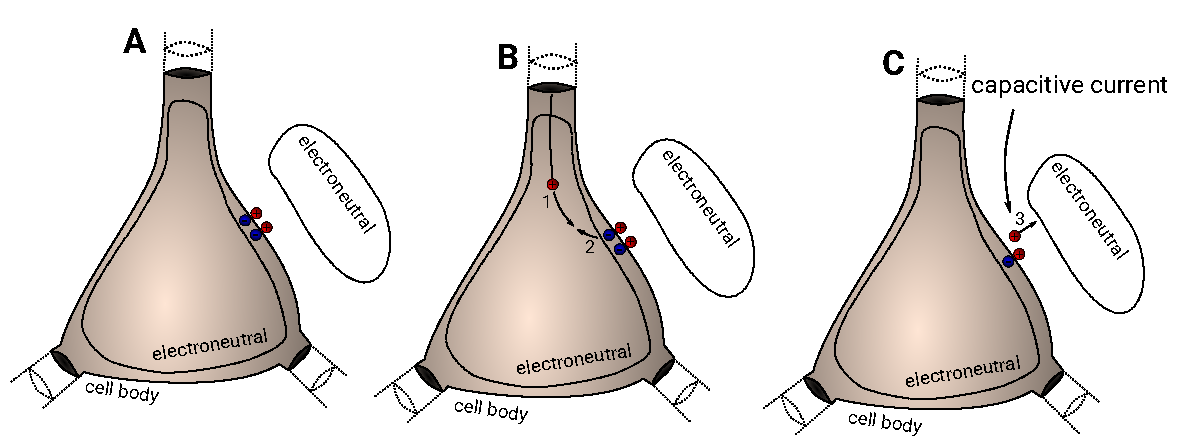
\includegraphics[width=1\textwidth]{capacitive_currents}
\end{center}
\caption{\textbf{Capacitive currents ensures current conservation.
\tvnnote{Mention time scale of this?}
\tvnnote{Not sure if this makes sense to include?}
}}
\label{fig:capacitive_currents}
\end{figure}

\subsection{Illustration with point-neuron model}
Consider for example the often-used point-neuron models \citep{Sterratt2011}. Since they have only one compartment, eq.~\ref{eq:current_conservation} demands that there should be no net transmembrane current, implying no extracellular potentials (see eq.~\ref{eq:VCtheory}). This means that, while point-neurons have an important role to play in investigating neural network dynamics \citep{Einevoll2019}, they are in general incapable of producing extracellular potentials (Fig.~\ref{fig:current_conservation}A; see however \cite{Mazzoni2015, Hagen2016}). 

\begin{figure}[h!]
\begin{center}
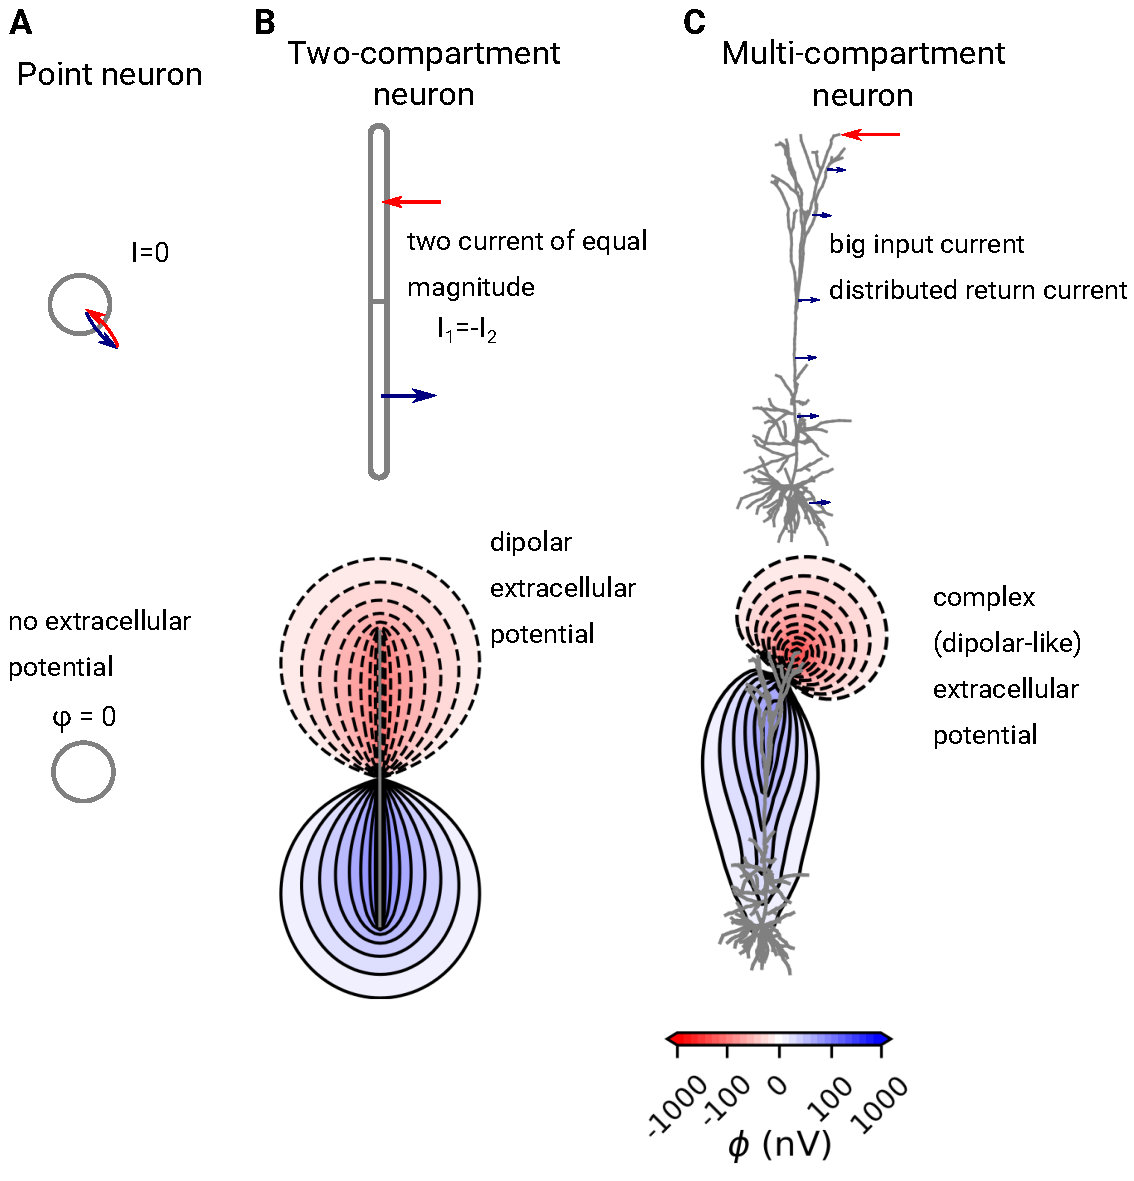
\includegraphics[width=0.6\textwidth]{dipoles}
\end{center}
\caption{\textbf{Effect of current conservation on extracellular potentials.} 
Illustration of synaptic input to three different types of cell models (top row), with the resulting extracellular potentials (bottom row). 
A: Point neurons have no net currents, and therefore cause no extracellular potentials. B: Two-compartment neuron models have two opposite currents
of identical magnitude, and cause dipolar extracellular potentials. C: Multi-compartment neuron models \citep{Hay2011} give rise to extracellular potentials with complex (but mostly dipolar-like) shapes.}
\label{fig:current_conservation}
\end{figure}


\subsection{Illustration with two-compartment model}
Consider now a cell model with two cellular compartments. Current conservation, through eq.~\ref{eq:current_conservation}, then implies $I_1 + I_2 = 0$, which in combination with eq.~\ref{eq:VCtheory} gives,
\begin{equation}
 \phi ({\bf r}) = \frac{I_1}{4\pi {\bf |r-r_1|} \sigma} + \frac{-I_1}{4\pi {\bf |r-r_2|} \sigma} = \frac{I_1}{4\pi \sigma}\left ( \frac{1}{{\bf |r-r_1|}} - \frac{1}{{\bf |r-r_2|}}\right ).
\end{equation}
In words, the exact same amount of current that goes into one compartment, goes out of the other, resulting in a current dipole (Fig.~\ref{fig:current_conservation}B).

\subsection{Illustration with multi-compartment cell model}
For multi-compartment cell models, the situation becomes more complex, but current conservation is still key in shaping extracellular potentials, and ensures that there are no current monopoles. This means that in general neural activity can be expected to cause both negative and positive currents, resulting in both positive and negative extracellular potentials (Fig.~\ref{fig:current_conservation}C).


\section{Local field potentials}

\ghnote{Suggest that we start these sections by explaining what $\phi$ tells us at this level. Also, we should refer to the VC-theory and explain which of the assumptions (1-6) that were relaxed in the specific case.}
\tvnnote{How much of an intro should we have here? If the Chapter intro has a broader focus and only refer to modelling of brain signals, we should have full LFP intro here.}

The Local Field Potential is the Low-Frequency Part ($\lesssim$ 500~Hz) of the extracellular potentials, and it is among the oldest and most used brain signals in neuroscience \citep{Einevoll2013}.
The LFP is expected to be dominated by large numbers of synaptic inputs to population of geometrically aligned neurons \citep{Nunez2006, Linden2011, Einevoll2013b}, and what determines a single neuron's contribution to the LFP is both the geometrical structure of the neuron, and the location of the synaptic inputs. 

Excitatory synaptic inputs opens small pores (ion-channels) in the cellular membrane of the post-synaptic cell, causing positive ions to flow into the cell \citep{Kandel2012}, which, by convention, is referred to as a current sink (negative current). As we have seen, this will necessarily lead to a current source somewhere else on the cell.  
Excitatory synaptic input to the apical dendrite of a pyramidal cell, will tend to give an apical current sink and a corresponding basal current source (Fig.~\ref{fig:dipole_basics}A), while excitatory synaptic input to the basal dendrite will give the opposite: a basal sink and an apical source (Fig.~\ref{fig:dipole_basics}B). Importantly, this means that excitatory input that simultaneously targets both the apical and the basal dendrite will give opposite source/sink patterns which will lead to substantial cancellation, and result in a much weaker contribution to the LFP (Fig.~\ref{fig:dipole_basics}C).
The same arguments also applies to inhibitory synaptic inputs, with the signs of the currents reversed (Fig.~\ref{fig:dipole_basics}D-F). 

Note that the LFP signature of apical excitatory synaptic input is inherently similar to that of basal inhibitory input (Fig.~\ref{fig:dipole_basics}, A versus E), and indeed, separating between cases like this poses a real challenge in enterpreting LFP signals [cite]. 

\begin{figure}[h!]
\begin{center}
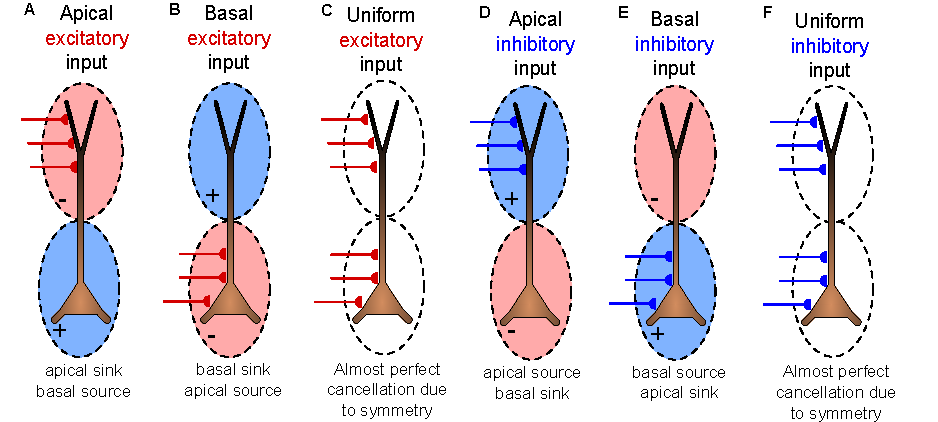
\includegraphics[width=0.8\textwidth]{dipole_basics}
\end{center}
\caption{\textbf{Basic building blocks of the LFP}}
\label{fig:dipole_basics}
\end{figure}



\begin{figure}[h!]
\begin{center}
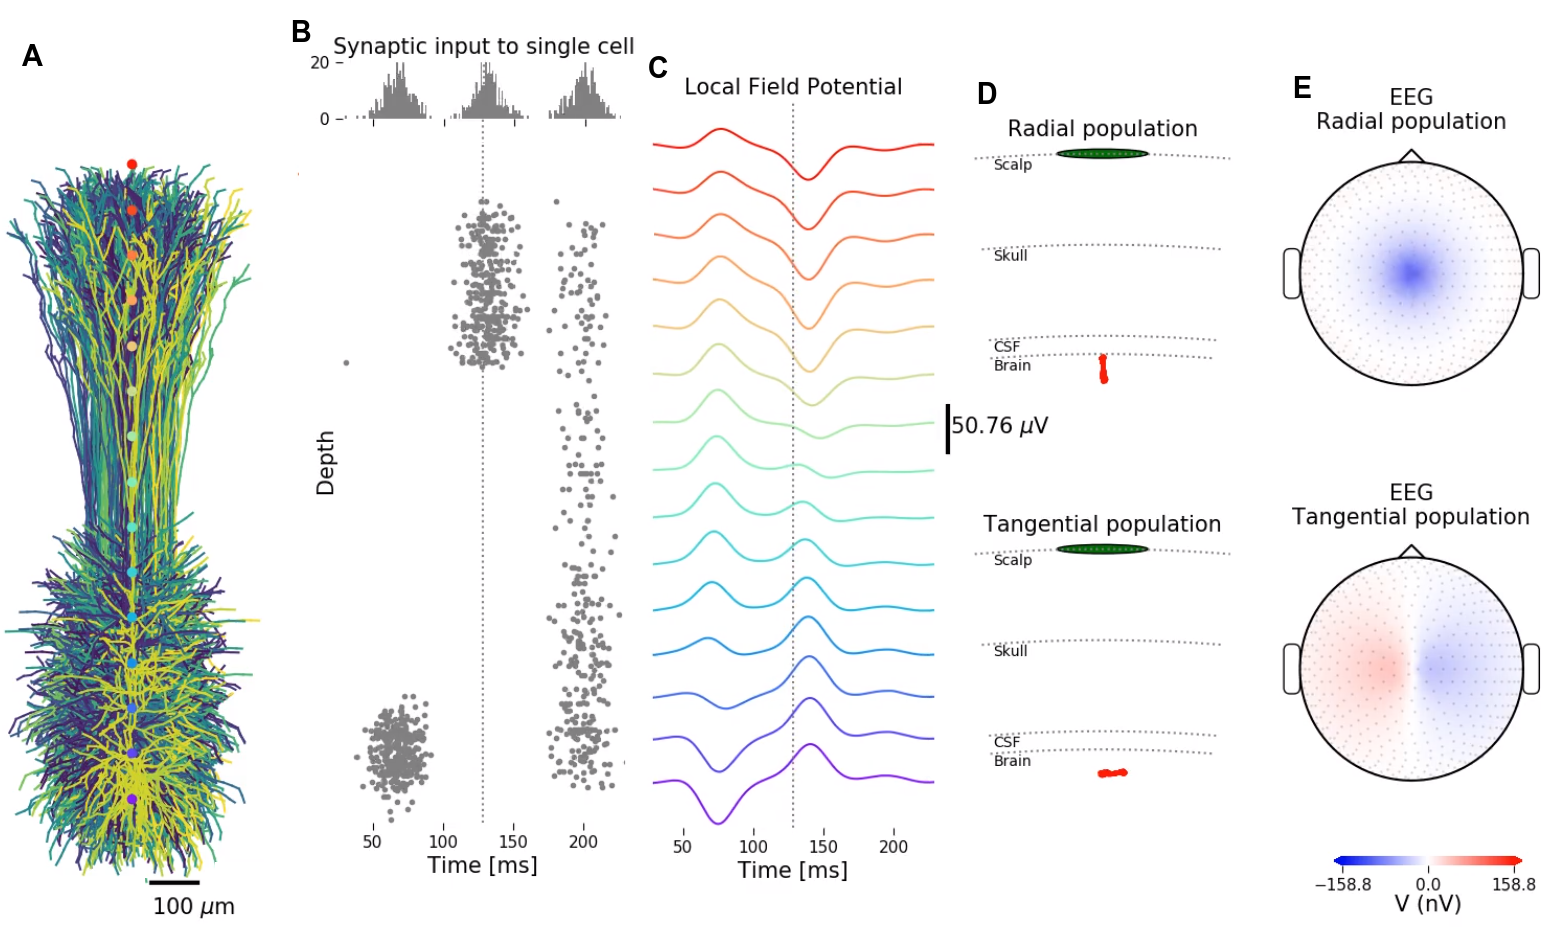
\includegraphics[width=1\textwidth]{population_EEG_MEG.png}
\end{center}
\caption{\textbf{[placeholder] LFP from different waves of synaptic input.}}
\label{fig:LFP_EEG_MEG}
\end{figure}

\subsection{Intrinsic dendritic filtering}

\subsection{Effect of spikes and active conductances}

Spikes are typically not expected to have an important role in shaping cortical LFP signals \citep{Einevoll2013, Haider2016}, but see also \cite{Reimann2013}.
However, highly synchronized spikes are expected to be very important for hippocampal sharp wave ripples \citep{Schomburg2012, Luo2018}. 

Subthreshold active conductances can also be expected to effect the LFP, and in particular the hyperpolarization-activated cation channel I$_{\rm h}$ might have a key role in shaping the LFP \citep{Ness2016, Ness2018}.

\cite{Suzuki2017} demonstrated that calcium spikes can also make sizable contributions to the LFP and ECoG signals, which opens up for exciting research opportunities, given the assumed important physiological role of such calcium spikes.


\section{MUA}
While LFPs are thought to mainly reflect the synaptic input to large populations, the multi-unit activity (MUA) can be used to probe the spiking activity. MUA can be used in combination with LFP to estimate the population dynamics, as for example in Laminar Population Analysis \citep{Einevoll2007, Blomquist2009}  

\section{ECoG, EEG and MEG}
\label{sec:EEG}
LFP signals are measured inside different brain structures, in the immediate vicinity of the current sources that are causing the LFP signals. A disadvantage with this is that it is invasive, in the sense that electrodes must be inserted into the brain tissue which can only be done in humans when there is a clear medical need, like for patients with intractable epilepsy [cite]. However, the current sources that are causing the LFP signals are also causing measurable signals at the brain surface, electrocorticography (ECoG), and at the outside of the head, called electroencephalograpy (EEG) for electric signals measured at the head surface, and magnetoencephalography (MEG) for magnetic signals measured outside the head (Fig.~\ref{fig:multimodal}).

Any combination of current sinks and sources can set up current multipoles \citep{Nunez2006}, and from electrodynamics we know that extracellular potentials at a distance $R$ from the source can be precisely described by a multipole expansion
\begin{equation}
\phi(R) = \frac{C_{monopole}}{R} + \frac{C_{dipole}}{R^2} + \frac{C_{quadrupole}}{R^3} + \frac{C_{octupole}}{R^4} + ...~.
\label{eq:dipole_expansion}
\end{equation}
Since current monopoles are unphysical due to current conservation, and the quadrupole, octupole and higher order terms are decreasing more strongly with distance $R$ than the dipole term, 

are negligible to the current dipole contribution when $R$ is sufficiently large, the extracellular potential from a neuron simulation can be estimated with the \textit{current dipole approximation} \citep{Pettersen2008, Pettersen2014, Nunez2006}:

No important signal filtering by head \citep{Pfurtscheller1975, Ranta2017}

\begin{equation}
\phi(\mathbf{r}) = \frac{1}{4 \pi \sigma} \frac{|\mathbf{p}| \cos \theta}{R^2}~.
\label{eq:dipole}
\end{equation}
Here, $\mathbf{p}$ is the current dipole moment in a medium with conductivity $\sigma$, $R = |\mathbf{R}|$, where $\mathbf{R}$ is the distance between the current dipole moment and the electrode location and $\theta$ denotes the angle between $\mathbf{p}$ and $\mathbf{R}$. As mentioned above, this approximation is applicable in the far-field limit, that is when $R$ is much larger than the dipole length $d$, $R > 3d$ or $4d$ \citep{Nunez2006}.

\subsection{Head models}
Can use analytic four-sphere (Fig. \ref{fig:head_models}A) \citep{Hagen2018, Naess2017}
Can also used pre-solved complex head models, like the New York head (Fig. \ref{fig:head_models}B) \citep{Huang2016}.

\begin{figure}[h!]
\begin{center}
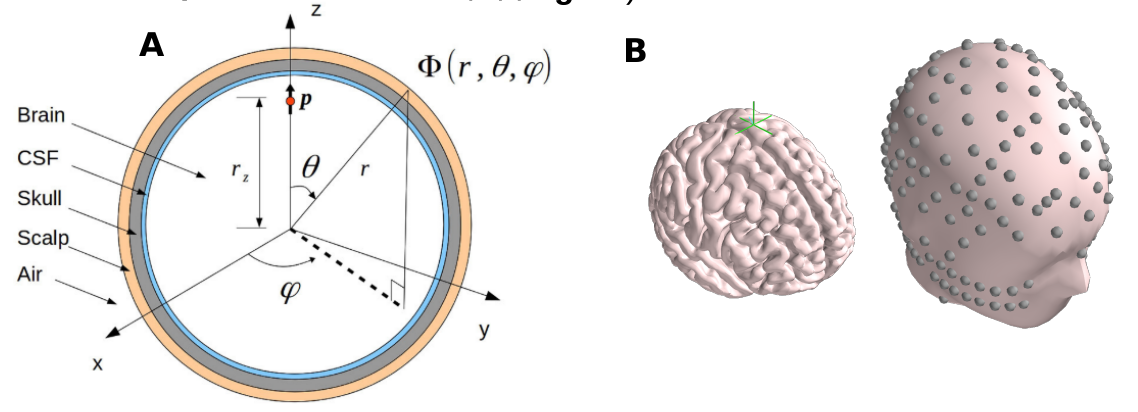
\includegraphics[width=1\textwidth]{head_models.png}
\end{center}
\caption{\textbf{[placeholder] Head models} A: Four-sphere. B: New York head model.}
\label{fig:head_models}
\end{figure}
\subsection{MEG}
Same same, but different. 
Much of what is said about electric signals also apply to the magnetic signals.

\section{Electrodes}
\tvnnote{Do we want this part?}
\subsection{Size}
Spatial averaging matters, but is relatively easily studied
\subsection{Frequency filtering}
Nelson says no (for recording electrodes) \citep{Nelson2010}

\section{Simulated test-data for benchmarking}
\tvnnote{Should we have this?}

Spike-sorting: \cite{Hagen2016, Buccino2019}

CSD: \cite{Pettersen2006, Potworowski2012, Ness2015}

Location and Cell type: \citep{DelgadoRuz2014, Buccino2018} 

LPA

\section{Other approaches}
Kernels \citep{Hagen2016}.
Proxies \cite{Mazzoni2015}

\section{Software tools}
LFPy etc.
\tvnnote{Recycle text from LFPy 2.0 paper about other softwares (sec 4.7.}

\section{Discussion}
\label{sec:discussion}
\tvnnote{Since it is textbook, should we rename to 'Summary'?}
\begin{enumerate}
 \item Summary of chapter
 \item Ongoing large-scale projects (HBP, Allen)
 \subitem Using LFP in constraining models?
 \item Brain-Machine interfaces?
 \item Where to go?
 \subitem fMRI, VSD, Ca img.
\end{enumerate}



%%%%%%%%%%%%%%%%%%%%%%%%%%%%%%%%%%%%%%%%%%%%%%%%%%
%%%%%%%%%%%%%%%%%%%%%%%%%%%%%%%%%%%%%%%%%%%%%%%%%%

\section{Acknowledgements}
\label{sec:acknowledgements}
This research has received funding from the European Union Horizon 2020 Framework Programme for Research
and Innovation under Specific Grant Agreement No. 785907 (Human Brain Project SGA2), the Research Council of Norway (Notur, nn4661k), and \tvnnote{INCF?}



%%%%%%%%%%%%%%%%%%%%%%%%%%%%%%%%%%%%%%%%%%%%%%%%%%
%%%%%%%%%%%%%%%%%%%%%%%%%%%%%%%%%%%%%%%%%%%%%%%%%%

\section{Bibliography}
\label{sec:bibliography}
\bibliography{ECS_bookchapter.bib}


%%%%%%%%%%%%%%%%%%%%%%%%%%%%%%%%%%%%%%%%%%%%%%%%%%
%%%%%%%%%%%%%%%%%%%%%%%%%%%%%%%%%%%%%%%%%%%%%%%%%%


\end{document}  
